\documentclass[12pt]{article}
\usepackage{fullpage}
\usepackage{graphicx, rotating, booktabs} 
\usepackage{times} 
\usepackage{fbb} 
\usepackage{natbib} 
\usepackage{indentfirst} 
\usepackage{setspace}
\usepackage{grffile} 
\usepackage{hyperref}
\usepackage{tikz-cd}
 \usetikzlibrary{cd}
\usepackage[export]{adjustbox}
\usepackage[most]{tcolorbox}
\usepackage{verbatimbox}
\usepackage{lscape}
\usepackage{afterpage}
\usepackage{amsmath}
\usepackage[labelfont={bf},textfont=it,labelsep=period]{caption}
 \usepackage{multirow} 
\setcitestyle{aysep{}}
\usepackage{dcolumn}

\hypersetup{
  colorlinks = true,
  urlcolor = blue,
  linkcolor = black,
  citecolor = black,
  pdfauthor = {Joshua Alley},
  pdfkeywords = {},
  pdftitle = {},
  pdfsubject = {},
  pdfpagemode = UseNone,
%  pdffitwindow = true
%  pdfcenterwindow = true
}



\singlespace
%\title{\textbf{Elections, Arms Deals and Autocratic Allies}}
\title{\textbf{Arms and Electoral Influence: How Arms Deals with Autocratic Allies Facilitate Defense Contracting in Swing States}}
\author{Joshua Alley \\
Assistant Professor \\
University College Dublin\thanks{Thanks to Brian Blankenship, Jonathan Caverley, Jonathan Chu, Ben Fordham, Erik Lin-Greenberg, Zachary Markovitch, Pieter Wezeman as well as participants in the Boston University Political Economy of Security Online Workshop Series and 2022 Meeting of the International Studies Association for helpful comments.} \\
joshua.alley@ucd.edu
}

 
\date{\today}

\bibliographystyle{apsr}

\usepackage{sectsty}
\sectionfont{\Large}
\subsectionfont{\noindent\large\textit}
\subsubsectionfont{\normalsize}

\makeatletter
\renewcommand\tiny{\@setfontsize\tiny{9}{10}}
\makeatother


\begin{document}

\maketitle 

\begin{abstract} 
Arms deals with U.S. allies, especially autocratic partners, facilitate swing state-focused defense contracting in the United States. 
U.S. leaders make arms deals to smooth defense contract awards in swing states.
Autocratic alliance prot{\'e}g{\'e}s have more need and political flexibility to strike arms deals near elections. 
I examine these claims by analyzing the electoral determinants of defense contracting and arms export deals by the United States. 
First, I  detail electoral cycles in arms deals between the United States and its allies. 
I then use prime contracting data to show that swing states receive more and less variable contract awards. 
Third, I employ Bayesian models to link defense contract awards around elections directly to arms deals and then examine sectoral differences in weapons deals and contracting.
The results suggest that.... 
\end{abstract} 


\newpage 
\doublespace 


\section{Introduction}



% US-Brazil 1972
In 1972, the Nixon administration struck ten different deals to transfer or sell arms to Brazil.
Over the next four years, Brazil's military dictatorship received 500 M-113 armoured personnel carriers, five destroyers, seven submarines, and eight S-2E Tracker anti-submarine warfare aircraft.
These deals came while Nixon sought reelection and subsequent deliveries continued after his 1974 resignation. 


% Obama 2012
Similar events took place in 2012, when Saudi Arabia ordered a large arms package from the Obama administration.\footnote{Obama first announced the deal in 2010.} 
Twelve deals included 400 Harpoon anti-ship missiles, 12 Apache attack helicopters for the Saudi National Guard, and 63 K-6 120mm mortars, along with parts for F-15 aircraft, guided bombs, and other helicopters. 
Deliveries of these systems and other weapons spanned the next eight years, including the 2015 Saudi intervention in the Yemeni civil war.\footnote{All deal information from \citep{Sipri2022}.}


% example- PBC consequences vary w/ security coop
These examples reflect a more general pattern, where electoral competition in the United States encourages arms deals with allies, particularly autocracies.
Arms deals help leaders use defense contracting to improve and stabilize economic conditions in electorally competitive areas \citep{Tufte1978, Mintz1988, Mayer1995, DerouenHeo2000, Becker2021}. 
In this instance, arms deals facilitate a high and stable flow of defense contracts to swing states, even as Congressional budgeting shifts. 
Electoral cycles in arms deals thus shape economic conditions and electoral competition. 


% arms exports logic
Alliance prot{\'e}g{\'e}s provide a key market for arms sales in part because leaders can justify transfers. 
Allies receive more arms from their patrons near elections because they control import decisions and receive security benefits. 
Autocratic allies are especially important because they receive more arms than other partners \citep{McManusYarhi-Milo2017} and autocrats have few constraints on accommodating electoral cycles.
%These arms export cycles reinforce cooperative relationships between U.S. leaders and alliance prot{\'e}g{\'e}s. 


% Findings
I scrutinize my argument connecting defense contracting, autocratic allies and arms export cycles in three steps. 
First, I examine how electoral competition shapes contract awards in an analysis from 2000 to 2020.
The first analysis finds that outside of war years, swing states receive more contracts and have less variation in prime contracting dollars. 
I then analyze U.S. arms deals from 1950 to 2019, and show that arms deals with autocratic allies increase as presidential elections approach, while dealmaking with democratic allies remains consistent. 
Finally, I connect the contracting and arms deals models in a joint model, and link deals and arms contracts within specific sectors.


% focus on the U.S.
The argument and analysis focus on the United States because it is a leading arms exporter, maintains expansive alliance ties, and there is prior evidence that leaders use defense contracting cycles for electoral advantage. 
While other countries with smaller economies and defense industries might behave in similar ways, deals and contracting cycles will be weaker or absent.
Regardless the pivotal economic and security roles of the United States make understanding the economic and security consequences of U.S. political budget cycles worthwhile.
Furthermore, other states might leverage security cooperation to facilitate different policy cycles. 


% economic and seucrity ties 
The argument and findings address three salient issues in international relations theory and practice. 
First, they reveal that efforts to manipulate domestic economic conditions with defense contracting have international security consequences. 
Just as domestic political business cycles in large countries like the United States reshape international economic exchanges and have knock-on effects in other countries \citep{Kayser2006, Kayser2009}, electoral competition alters security cooperation. 


% coercion
Second, this paper provides new insight into alliance bargaining and statecraft. 
Scholars often address coercion and divergent preferences in alliances \citep{Oatley2015, Beckeretal2023}. % \citep[pg. 122]{Oatley2015}
But as \citet{Baldwin2020} notes, statecraft includes positive inducements and negative sanctions. 
This paper highlights positive statecraft by alliance prot{\'e}g{\'e}s, who use arms deals to cooperate with their patron.
As a result, it connects with prior work on issue linkage in alliance management, including studies of alliance formation \citep{Poast2012} and credibility \citep{Davis2008, Poast2013}.
In this instance, patron leader and prot{\'e}g{\'e} incentives align.


Finally, my results complement prior findings that foreign states' economic policies impact electoral competition. 
\citet{KimMargalit2021} find that Chinese tariffs reduced Republican vote share in the 2018 midterm elections by targeting industries in competitive districts.
In the same way, \citet{ChyzhUrbatsch2021} find that Chinese soy tariffs hurt Republican congressional candidates in soy-producing areas. 
My argument inverts these findings by examining how security cooperation facilitates electoral budget cycles and helps incumbents. 
As a result, small states exert big indirect influence on alliance patrons \citep{Keohane1971}.


% need an outline 
The paper proceeds as follows. 
To start, I outline an argument detailing the international consequences of political business cycles in the United States, the role of defense contracting in those cycles, and the consequences for arms deals. 
I then test the process in three steps. 
First, I model the mean and variance of contract awards as a function of electoral competition to show that swing states have larger and more stable defense contracting flows. 
I then demonstrate that arms exports from the United States to allies increase more as presidential elections approach.
Third, I estimate a joint Bayesian model of the process and link contracts with deals for specific weapons.
The last section discusses the results and offers concluding thoughts.


\section{Argument}


This argument explains how international arms deals facilitate domestic political budget cycles.
First, I detail constraints on aggregate budget cycle tools.
I then discuss how presidential control and Congressional influence makes defense contracting an attractive way to manipulate economic conditions. 
Arms deals with allies can accelerate efforts to target defense contracting awards to competitive areas. 
Among U.S. allies, autocracies with few constraints on their leaders and strong security motivations to curry favor by accepting arms are especially likely to make arms deals around elections.


Electoral considerations impact policy \citep{Nordhaus1975}.\footnote{See \citet{Dubois2016} for a review of the vast political budget cycle literature.} 
When leaders want to win office, they can use policy tools to bolster economic growth and win over voters. 
Leaders create political budget cycles by using fiscal and monetary policy to increase economic growth near elections and retain power for themselves or their party \citep{Tufte1978, Rogoff1987}. 
The composition and magnitude of these cycles varies. 
For example, strong central bank interdependence and fixed exchange rates make fiscal cycles more likely \citep{ClarkHallerberg2000}. 
%Even some independent central banks exhibit modest cyclical behavior, however \citep[pg. 247]{Dubois2016}


How leaders bolster economic growth vary with national political institutions. 
Federal Reserve independence limits political influence on monetary policy in the United States, for instance.\footnote{Both Lyndon Johnson and Donald Trump had limited ability to browbeat Federal Reserve Chairs into changing monetary. 
Johnson sought looser monetary policy before the 1968 presidential election, but Fed Chair William McChesney Martin continued to tighten policy.
Trump's tweeted demands for looser monetary policy to increase growth before the 2020 election similarly had little impact on Jerome Powell.}
Recent scholarship emphasizes specific policy cycles because leaders struggle to manipulate aggregate economic instruments where they have more direct influence. 
In fiscal policy, aggregate budgets often give leaders limited spending discretion.


Limited flexibility with aggregate instruments encourages democratic leaders to use targeted policies.
Targeting maximizes the electoral impact of finite resources.
Many spending shifts can be narrowly tailored \citep[pg. 248]{Dubois2016}.
Leaders also employ other policies such as trade disputes \citep{Conconietal2017}, labor agreements \citep{Ahlquist2010} and land reform \citep{Philips2020} to win support in key constituencies.


% Defense spending/contracts as flexible instrument
Scholars have long speculated that defense spending is a useful instrument for budget cycles (e.g. \cite{Tufte1978, Mintz1988}).
Executive leaders often have more discretion in defense resource allocation, and defense spending has economic ramifications.
\citet{WhittenWilliams2011} note that defense spending can serve social welfare goals and \citet{Becker2021} finds that unemployment in NATO members encourages leaders to shift spending from equipment to personnel.


% in US context, contracts
Recent studies in the United States argue that defense budgets are poor political tools, however, as Congress makes allocations two years ahead.
This shifted attention towards defense contracting, as leaders control contract timing and disbursement \citep{Mayer1995, DerouenHeo2000}.
Giving contracts also allows leaders to focus on key constituencies and claim credit for awards \citep{DerouenHeo2000}. 
Leaders generally target spending changes near elections to electorally important areas like swing states \citep{KrinerReeves2015}, and spending increases support for incumbents \citep{KrinerReeves2012}.


% seeking stability
When awarding defense contracts, leaders do not want political cycles, however. 
Rather, I argue that leaders seek high and stable contracts in electorally competitive areas like swing states. 
Large year to year changes in defense contracting could antagonize key constituencies. 
Firms and local business leaders could decry unstable contracting that complicates year to year planning. 


% maintaining stability is more important near elections 
Ensuring high, stable contracting in swing states is more important near elections. 
All else equal, leaders will be more willing to risk criticism for defense contracting variance when they will no immediately face voters. 
Smoothing contract awards becomes more urgent as elections approach, but the budget process does not accommodate this. 


% demand
The Congressional budget process sometimes hinders year to year contracting stability. 
Leaders can allocate contracts within the budget, but finding additional funds is harder. 
Most defense programs operate on annual budget allocations.
Congress rarely authorizes multi-year procurement (CITE CRS HERE). 
As a result, program disbursements can vary from year to year, especially for smaller outputs like munitions and missiles. 


Moreover, when leaders want to award contracts to swing state firms, the U.S. military may lack absorption capacity to incorporate outputs.
Increased supply for defense contracting does not respond to military demand.
This makes finding other buyers who are less constrained by the U.S. budget process a critical task.


When leaders seek increased defense contracting, foreign markets are an alternative source of demand.
Either foreign countries can take new production, or U.S. leaders can sell or transfer old equipment to partners to make room in U.S. stocks. 
Using defense contracting for political gains thus has international spillovers.\footnote{% Political Business cyles
Other work examines the international economic consequences of budget cycles.
Fiscal and monetary policy shifts impact currency prices and economic growth, which then alters trade and financial ties. 
Economic interdependence leads to correlated economic growth across countries \citep{ArtisZhang1999, Kayser2006} and increases the global economic influence of large economies. 
\citet{Ito1991} finds that U.S. elections increase economic growth in Japan, while \citet{ThompsonZuk1983} uncover some evidence of similar cycles in advanced industrial economies.
\citet{FoersterSchmitz1997} argue that U.S. electoral cycles impact international stock returns.
}


% timeline and intermediate goods
Crucially, leaders only need deals and confirmed orders to start up defense contracting. 
Final transfers can come years later, and do in many cases. 
Arms export deals are more likely to follow electoral cycles than transfers of finished products, as production times for defense goods vary widely. 
Large platforms like ships, tanks and warplanes can take years to assemble, while munitions and smaller platforms take less time. 


% scope condition- peace years
Efforts to provide high and stable contracts for swing states are more salient in peacetime. 
During active conflict, elevated demand for munitions, platforms and other arms creates substantial contracting across all states. 
Leaders thus have less need to focus contracts, and less scope to do so.   


% additional production and foreign markets
%When defense production and planning diverge, foreign markets provide alternative takers for excess arms production from defense contracting cycles. 
When U.S. leaders attempt to use arms deals for defense contracting, not all countries are useful partners. 
U.S. allies are more likely to take arms exports than other states. 
Security partners are a pivotal outlet because alliances facilitate security, economic and political cooperation.
The United States often transfers or sells arms to alliance prot{\'e}g{\'e}s, and some allies have means and motivation to strike arms deals at helpful points in the electoral cycle. 



\subsection{Alliances and U.S. Arms Deals}


% basic asymm alliance framework
Asymmetric alliances between large and small states, like those between the United States and its allies, are grand bargains.
In general larger patrons protects smaller prot{\'e}g{\'e}s in exchange for foreign policy concessions \citep{Morrow1991}.
While patrons increase their foreign policy influence, junior alliance members garner protection from external threats and sacrifice some foreign policy autonomy.


%Electoral cycles in arms exports to allies benefit U.S. leaders.
%Presidents gain capacity to manipulate economic conditions with defense contracting and signal support for U.S. alliance prot{\'e}g{\'e} s by sending arms.
%Defense contracting cycles increase prosperity in key electoral areas, which increases a leader's odds of winning office for themselves or their party.\footnote{\citet{Yarhi-Miloetal2016} argue that arms transfers sometimes substitute for formal alliances so patrons can provide security while managing entrapment risk.}


% potential markets: allies
% take new or used stuff to make room
U.S. allies are an obvious market for deals to feed defense contracting, in part because established channels reduce start-up costs and facilitate cumulative deals.\footnote{I focus here on formal and informal allies, because formal treaties like NATO are not the only U.S. security commitments. Taiwan, Israel and Saudi Arabia have informal security guarantees and often receive U.S. arms. \citep{Yarhi-Miloetal2016}}
\citet{Thurneretal2019} find that while the relative importance of security and economic factors fluctuates, alliances consistently increase arms transfers.
Common security interests and economic integration of defense industries create economic and security ties that encourage arms trade \citep{Bitzinger1994}. 
Defense industry integration generates trade in intermediate defense goods \citep{Brooks2005}. 
U.S. allies use weapons, systems and doctrines that facilitate deals for additional arms. 


% less export cycles to non-allies
% each evidence sentence could be its own paragraph 
Allies are more likely than other states to make arms deals, and autocratic allies are especially likely to make arms deals near elections. 
The security externalities of arms transfers constrain electoral cycles in arms exports to non-allies. 
U.S. elites will be less willing to increase the capability of states with fewer common interests, even if it facilitates contracting cycles.


Competing elites are also more likely to object to arms deals outside alliances.
Leaders could face electoral costs if other elites publicly criticize a deal \citep{Saunders2022}.
Arms transfers to non-allies could face greater opposition scrutiny near elections, leading presidents to forestall criticism by forgoing contentious transfers.
Limited defense industry cooperation further constrains exports outside alliances, while allies with defense industrial ties can receive intermediate goods as well.


% positive statecraft tie-in from Baldwin 
Allied leaders also benefit from arms deals around elections, because deals curry favor with an alliance patron, bolster military capabilities and deepen perceived commitment.
Helping patron leaders with arms deals will dispose them more favorably towards an ally. 
Allies increase their military capabilities with new arms as well, which can make their fighting forces more effective. 
Finally, allies gain confidence in their patron's commitment when deals become deliveries because arms exports are a costly signal \citep{McManusYarhi-Milo2017}.


Arms deals are therefore positive statecraft by allies. 
States often use purchases and transfers to increase their political influence \citep[pg. 42-3]{Baldwin2020}.
\citet[pg. 184-5]{IkenberryGrieco2003} note that states often use direct transfers to attract and sustain security commitments.  


% Sales and transfers- who pays for what
Moreover, prot{\'e}g{\'e}s do not always pay for U.S. arms.
The United States often subsidizes or gifts arms transfers through foreign military sales programs. 
While these still count as arms exports, they impose few immediate costs on recipients.
Alliances make such subsidized transfers easier to justify to other elites, as they promote common security interests. 


\subsection{Arms Deals with Autocratic Allies}


While all allies could benefit from U.S. arms, autocratic allied leaders are more likely to make arms deals near elections. 
Autocracies both the means and motivation to make arms deals.
These leaders have fewer domestic political constraints, which increases their budget and policy flexibility. 
They also have stronger security motivations to use arms deals to improve relations with the United States, because arms transfers are central to U.S. security guarantees to autocracies.


% to work, allies must have pol  and budget flexibility
Allied leaders must have the political freedom to make arms deals.
Governments are the customer for most arms sales or transfers, so they generally have some latitude to take arms.\footnote{This mirrors how political control of firms increases trade policy flexibility \citep{Davisetal2019}.}
At the same time, not every regime is equally free to make arms deals. 


% constraints
Autocratic allies of the United States have greater political flexibility to make arms deals around elections than democracies. 
Democratic leaders who might face media or elite scrutiny of deals for U.S. arms.
Media or elites might object to spending on arms, competition for domestic arms manufacturers, or excessive alignment with the United States.


Autocrats are less constrained.
Even if other domestic actors in an autocracy are opposed to additional outlays on U.S. arms, they have few ways to constrain the leader.\footnote{This changes when opponents of U.S. arms deals are part of the autocrats power base.}
Media scrutiny of deals is also less likely to occur or challenge an autocrats power base. 


% offstage signaling and need
Autocrats also strike deals to bolster their security.
Arms transfers are more central to credible U.S. commitments to autocracies.  
The United States prefers ``offstage'' signals of support for autocrats, rather than public demonstrations of commitment \citep{McManusYarhi-Milo2017}.
Arms transfers are a pivotal offstage signal and sometimes substitute entirely for formal security guarantees \citep{Yarhi-Miloetal2016}. 
When arms are the core of how the U.S. provides security, autocrats will be more willing to make arms deals that increase military capabilities and signal continued alignment with the United States.


% further need- no ideological affinity
Autocrats also have fewer other tools to curry favor with U.S. leaders.
Formal alliances might promote democratization \citep{GiblerWolford2006, Warren2016}.
The U.S. public dislikes alliances with autocracies \citep{Alley2022}, so autocrats have less capacity to pursue deeper ties in other areas. 
The net result is that arms deals are central to U.S. ties with autocratic security partners, so autocrats are more likely to make arms deals near elections. 


% deliberate or not?- key for statecraft argument. 
This argument is agnostic about whether allies make a conscious decision to help political budget cycles by making arms deals.
While they want improve their alliance relationship, U.S. allies need not choose to accommodate electoral cycles in defense contracting.
Allies may receive better terms and more financial support to take additional goods, or take transfers or surplus materiel as a deliberate favor to leaders who have supported their foreign policy interests. 


% objection- more scrutiny of deals around elections
A potential objection to this argument is that striking arms deals with autocrats might be more costly near elections for U.S. leaders, because political opponents could criticize them for it. 
In this telling, opposition elites can make arms deals a more ``front stage'' signal than U.S. leaders would like. 
Even if this applies, U.S. leaders may still benefit, as arms deals provide concentrated benefits, while alliance critics are more diffuse.\footnote{Another reason this may not work is that deal announcements sometimes precede final orders by years.}
Opponents thus face collective action problems that beneficiaries of deals and corresponding contracts do not. 
When contracts focus on electorally salient areas, leaders can expect that the benefits outweigh any costs. 



%The overall argument process is as follows.
%As elections, leaders are more likely to award defense contracts to electorally competitive areas. 
%In addition to this direct path, U.S. leaders also strike arms deals with other states, to generate further contracts. 
%Electoral cycles in defense contracting follow.  


%\begin{figure}[htpb]
%\centering
%\begin{tikzcd}[ampersand replacement=\&]
%                                                                     \& |[alias=D]| \mbox{Arms Deals with Autocratic Allies}  \arrow[d]  \\                                                                    
%\mbox{Time to Election} \arrow[bend left = 10, to = D] \arrow[r, to = Y]     \& |[alias=Y]|    \mbox{Defense Contracting}   
%\end{tikzcd}
%\caption{Summary of the argument process linking election timing to cycles in U.S. arms deals and defense contracting.}
%\label{fig:arg-process}
%\end{figure}


% Result- increased exports, tied to electoral cycles
The result of this process is high and stable defense contracting in swing states.
This expectation diverges from classic electoral cycles arguments that emphasize new policies near elections. 
One way leaders ensure this is by striking more arms deals as elections approach, especially with autocratic alliance prot{\'e}g{\'e}s.
Arms deals thus shape electoral competition in the United States. 



\subsection{Implications}



The argument generates several testable implications, about U.S. alliances, arms deals and defense contracting. 
Again, this argument applies best and perhaps exclusively to the United States.  
Arms deal cycles and defense contracting in swing states are the result of a large defense industry, many security commitments and the peculiarities of the electoral college. 
Fixed election scheduling further reduces endogeneity between policy decisions and election timing. 
Other leaders may behave in similar ways within their specific electoral institutions, however. 


The first hypothesis predicts electoral cycles in arms deals, especially to autocratic allies.
Democratic allies will be less likely to make cyclical arms deals. 
As a result, greater proximity to presidential elections will increase arms deals with autocratic allied states. 


\begin{quote}
\textsc{Arms Deals Hypothesis: As time to a presidential election decreases, U.S. arms deals with autocratic allies will increase.}
\end{quote}


The second prediction deals with electoral competition and contract awards. 
Because leaders are using contracts to increase their odds of winning election, greater electoral competition in a state should lead to more prime contract awards.
Electoral competition should also encourage leaders to smooth defense contracting over time, which reduces contracting variance in swing states. 
This is most important during peacetime because conflict stimulates large contract disbursements without reference to electoral geography. 
 

\begin{quote}
\textsc{Defense Contracts Hypothesis: Outside of conflicts, swing states will receive more prime defense contract awards and have lower variation in contract awards than other states.}
\end{quote}


Finally, I expect that arms deals help stabilize prime contract awards in swing states.
By striking deals, leaders can focus contracts in key districts that might otherwise lose out in the regular budget process. 
Established arms manufacturing in key electoral areas facilitates this process. 


\begin{quote}
\textsc{Deals and Contracts Hypothesis: As arms deals increase, variance in swing state contract awards will decrease.}
\end{quote}


% What's next
In the following, I examine each of these hypotheses. 
In the first analysis, I use a series of descriptive data and single-outcome statistical models to illustrate each step in the process.
This starts with descriptive data on defense contracting from 2000 to 2020, then shows how arms exports to allies track U.S. electoral cycles, and ends with a model of electoral cycles in U.S. trade. 
After that, I test the third deals and contracts hypothesis by unifying the different outcomes in Bayesian model.
The joint model captures the process whereby arms deals increase the association between electoral competition and defense contracting awards. 



\section{Arms Transfers and Presidential Elections}


The arms deals hypothesis predicts electoral cycles in U.S. arms deals with autocratic allies.
To test this hypothesis, I model U.S. arms deals from 1951 to 2014 using deals data from the SIPRI Arms Transfer Database \citep{SIPRI2021}.
The outcome in this panel dataset of all states outside the United States is the annual count of deals, based on SIPRI's trade register. 
This section presents count data regression estimates of annual arms deals. 


% Why focus on deals
I analyze arms deals rather than observed arms transfers for three reasons.
First, elites can announce arms deals and related contracts immediately. 
Secondly, deliveries can take years after a deal is announced, even for second-hand or aid transfers of existing equipment. 
Finally, deliveries often space out the total value of a shipment over several years, especially for deals with many weapons or larger platforms. 


% key independent variables- ally/partner, 
The argument suggests that three variables driving U.S. arms deals. 
The first is electoral competition, which I measure with an indicator of the number of years to a presidential election. 
The second key factor is whether a country is a U.S. ally. 
I measure alliance status with a binary indicator of whether a country is a formal U.S. treaty ally using data from the ATOP project \citep{Leedsetal2002}, as well as one of three states that have not always had a formal treaty commitment but are widely seen as U.S. allies with implicit security guarantees; Israel, Taiwan and Saudi Arabia. 
I include informal allies because in some of these cases arms substitute for a formal alliance, but the United States is still attempting to ensure partner security \citep{Yarhi-Miloetal2016}. 
Finally, I measure country democracy using the VDem project's polyarchy measure \citep{Coppedgeetal2008}. 
I interact all three of these variables to predict arms deals. 


% models
To estimate how alliances, democracy and election timing shape arms deals, I use a Poisson model.
This fits the annual count of arms deals well.
To preserve compatibility with a later joint model, I use Bayesian estimation with the brms package for \textsf{R} \citep{Buerkner2017}. 
I show in the appendix that using a Gaussian outcome gives similar inferences. 


Along with the three key independent variables, I adjust for other factors that are correlated with arms deals, alliances, and democracy. 
The first control variable is a binary indicator of Cold War years, as more U.S. allies were autocratic during this period. 
I also adjust for EU membership as a potential constraint on some states. 
Further country-level controls include logged GDP, population, and distance the from United States, as well as a binary indicator of common language. 
Finally, I adjust for presidential partisanship with a dummy indicator of years with a Republican president.  



\subsection{Results}


Because interpreting coefficients in triple interactions is challenging, I summarize the interaction of alliances democracy and presidential election proximity in \autoref{fig:us-arms-plots}.\footnote{See the appendix for coefficient estimates.}
This figure plots predicted arms deals based on proximity to an election and whether a state is a U.S. ally or not. 
Each facet sets recipient democracy at the minimum, first quartile, median, third quartile and maximum.


\begin{figure}[htpb]
	\centering
		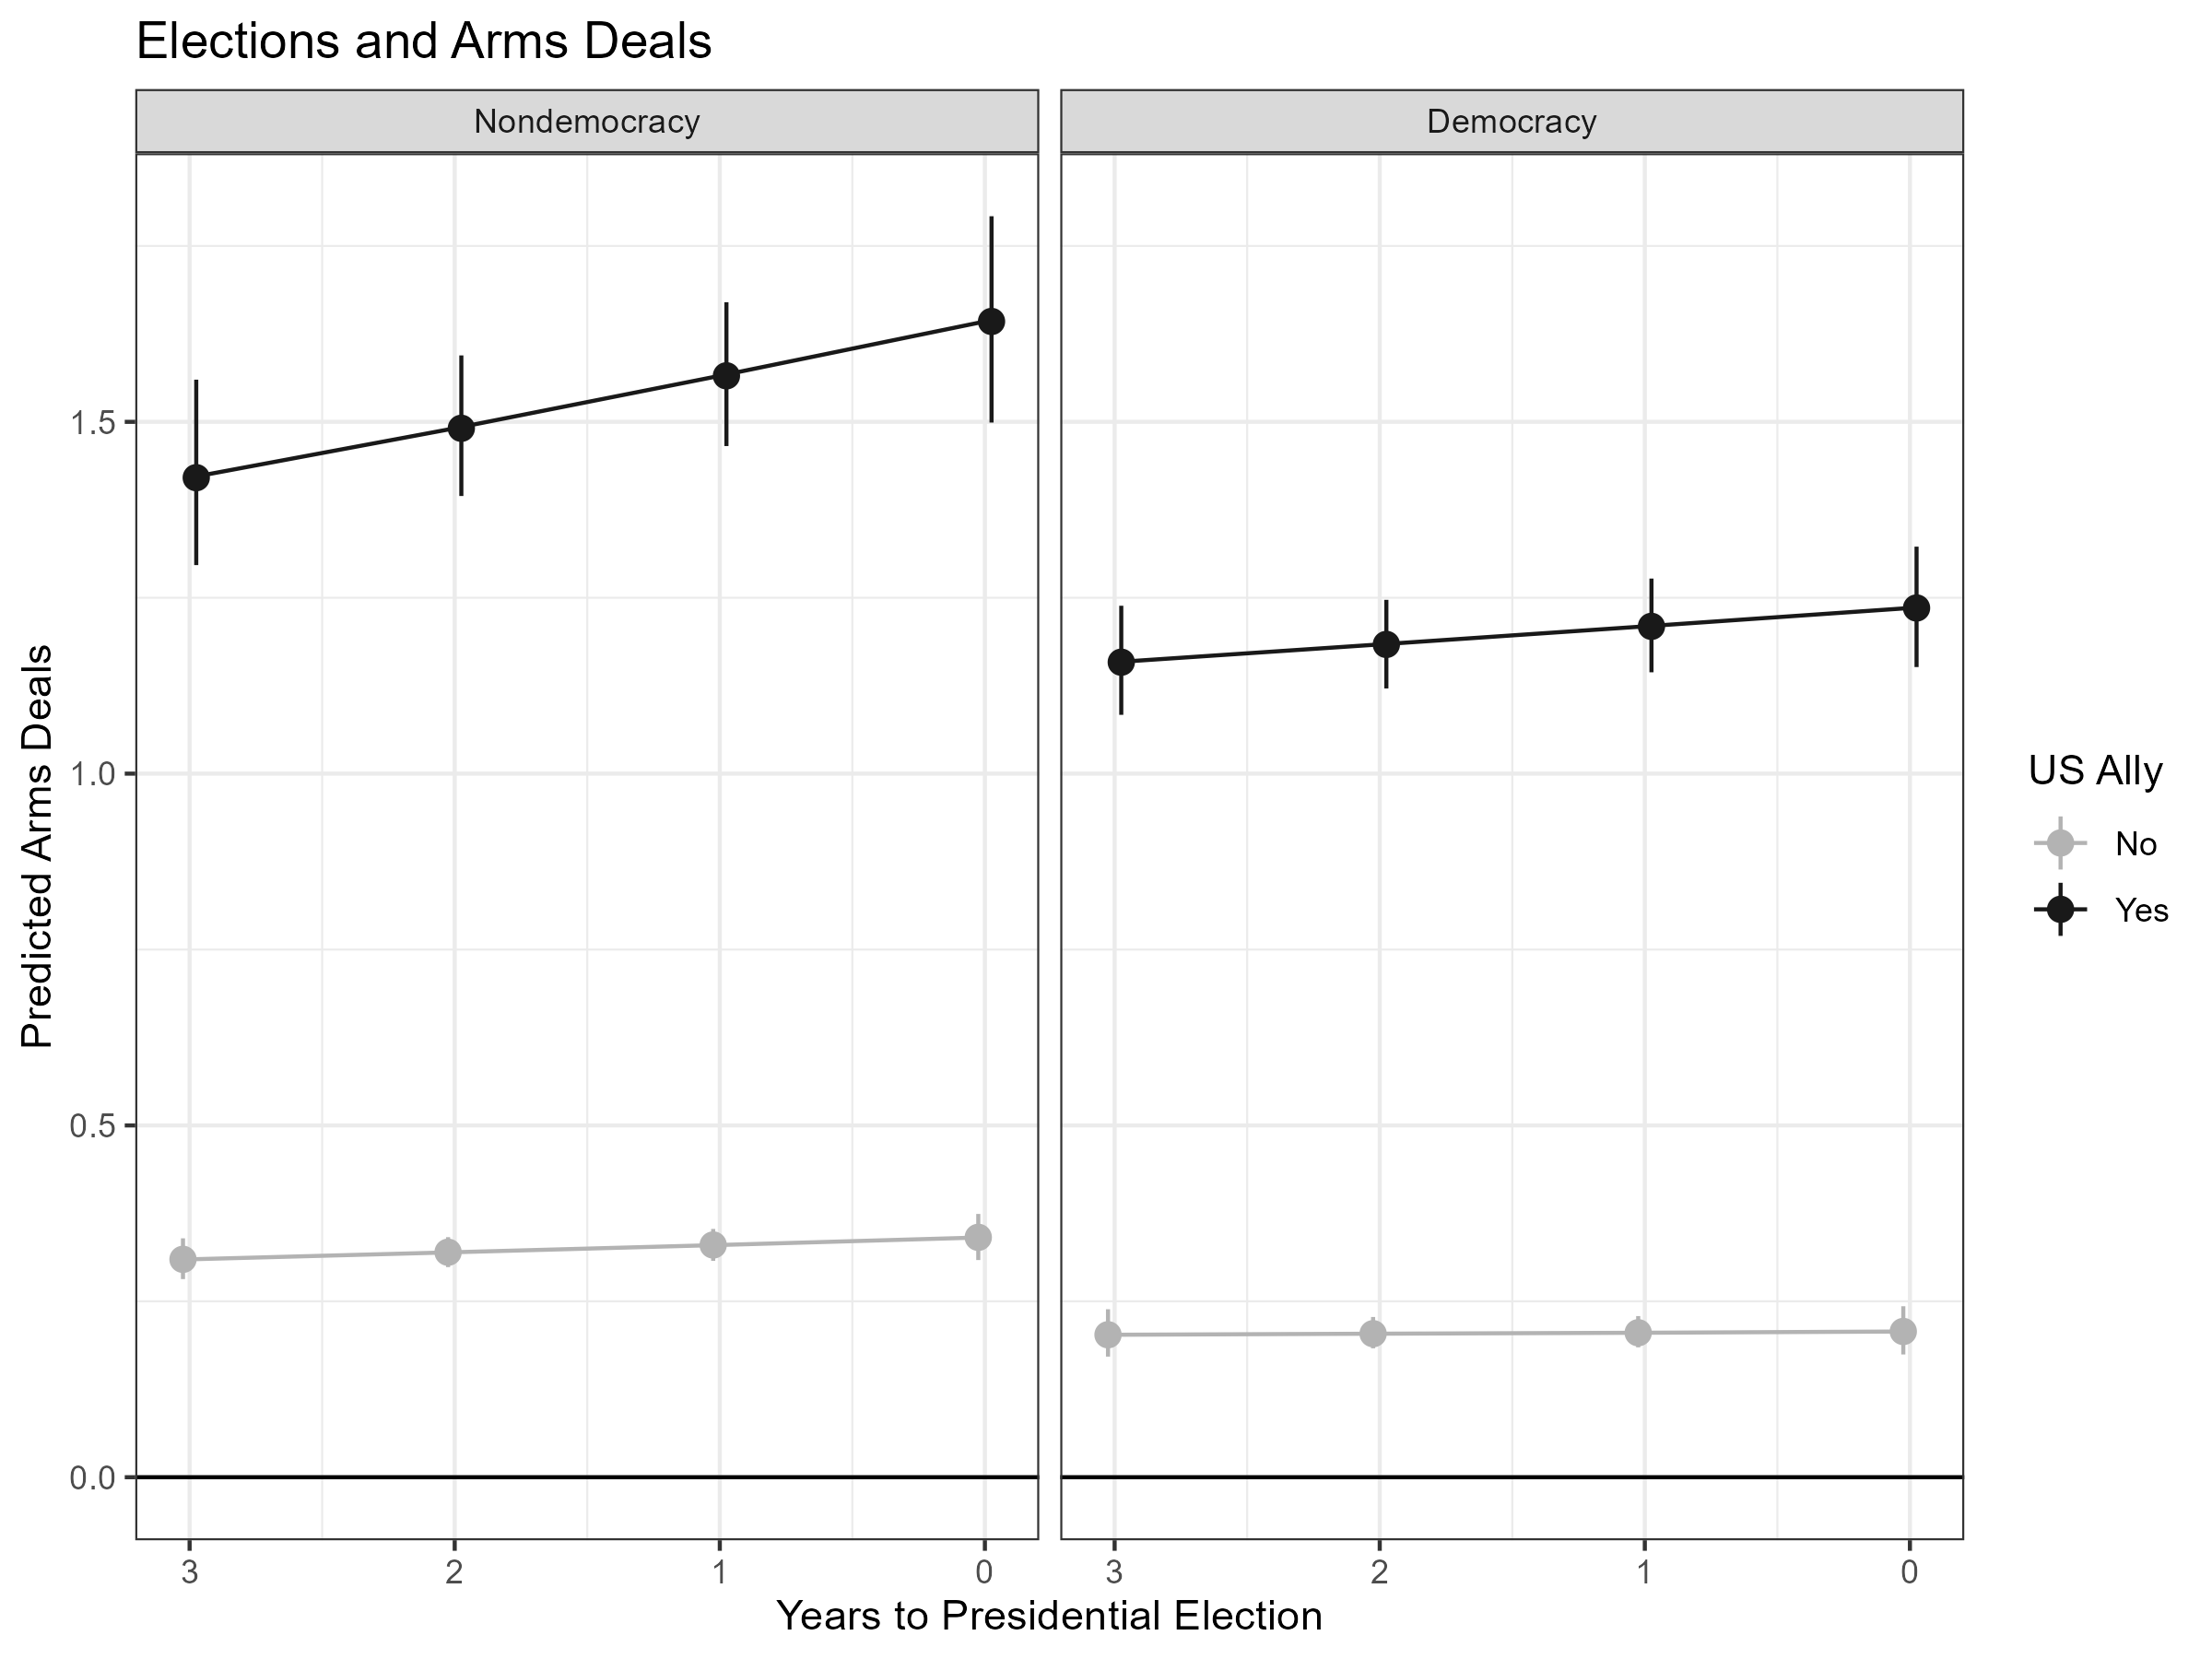
\includegraphics[width=0.95\textwidth]{../figures/us-arms-plots.png}
	\caption{Predicted arms deals between the United States and other states 1950 to 2014 based on presidential election proximity, democracy, and security alliances. Points mark the estimates and error bars summarize the 95\% confidence interval.}
	\label{fig:us-arms-plots}
\end{figure}


There are two key inferences in \autoref{fig:us-arms-plots}.
First, the United States makes more arms deals with allied states than non-allied states, regardless of regime type. 
Predicted deals with non-allied states are low and basically constant across the different levels of democracy. 
The impact of an alliance on arms deals is much greater for autocracies than democracies, however, which is consistent with \citep{McManusYarhi-Milo2017}. 
U.S. allies with minimal polyarchy scores receive one more arms deal a year than states with similar democracy, all else equal. 
Fully democratic U.S. allies receive .4 deals more in expectation. 


The second inference is that electoral cycles in arms deals are present for autocratic allies and absent for democratic allies.
When allied polyarchy is at the minimum value, predicted arms deals rise from 1.6 to 1.95 throughout the presidential election cycle.
Hypothesis tests of equality between allied arms deals at minimum democracy at each level suggest that the increase of .8 deals in each year of the electoral cycle is difference is clearly positive. 
The electoral cycles when democracy is at the 1st quartile or median are also clearly positive, but are much less substantively important.
This cycle diminishes as allied democracy increases, so fully democratic partners see no change in arms deals as elections approach.  


Electoral cycles are only present for autocratic allies. 
States that are not US allies do not change arms deals throughout the electoral cycle. 
Alliances increase the level of arms deals, and regime type impacts responsiveness to presidential elections. 


These estimates support arms deals hypothesis. 
As presidential elections approach, arms deals rise, but only with autocratic allies. 
Arms deals with democratic allies are unchanged by electoral competition.


These arms deals with autocratic allies near elections are connected to electoral cycles in defense contracting. 
If there are no cycles in defense contract awards, then arms deals have less tangible consequences. 
The next analysis checks for electoral cycles in defense contracting awards. 



\section{Electoral Competition and Defense Contracting}


To show the electoral correlates of defense contracting, I use Department of Defense prime contract award data from the USAspending.gov database.\footnote{Link here: \url{https://www.usaspending.gov/download_center/custom_award_data}.} 
This archive contains data on individual contract awards starting in the 2000 fiscal year, and I collected all Department of Defense contracts from 2000 to 2020.
The key outcome is the log of total defense contracts tied to arms production awarded to a state in every year.\footnote{This measure excludes other contracts besides weapons production because arms deals are unlikely to translate into other contracts.}


The key independent variable identifies swing states in presidential elections. 
Following \citet{KrinerReeves2015}, I code swing states as those where the losing party won at least 45\% of the two-party vote in three straight elections. 
Core states are those where the President's party received more than 55\% of the two-party vote. 


Because swing states only receive more contracts during conflict, I must account for the Global War on Terror, which increased defense spending through wars in Afghanistan and Iraq.  
To do this, I include an indicator of peak years in the global war on terror, which is one from 2001 to 2011, and zero otherwise.\footnote{I end the peak years at 2011 with the U.S. withdrawal from Iraq.} 
I then interact this dummy with the swing state indicator. 
The three dummies thus have non-swing states after the global war on terror as their reference category. 


In addition to the electoral competition and war variables, I include three controls. 
First, I adjust for population and GDP, in case larger and more prosperous states receive more contracts. 
The final control adjusts for presidential partisanship by coding years with a Republican President with one. 


The final adjustments in the model account for clustering and temporal dependence.
First, I include state and year varying intercepts because observations cluster at these levels. 
Current contracting also depends on past contracting, as the defense industrial base is concentrates in particular areas and moving is difficult. 
I therefore include a state-specific lagged dependent variable, which allows temporal dependence in contracting to vary by state. 


% describe the model 
To test the defense contracts hypothesis, I must estimate the impact of swing state status on the mean and variance of defense contracting. 
To do this, I fit a Bayesian distributional model where electoral competition predicts the mean and variance of annual defense contract awards.\footnote{Model specified and estimated with \textsf{brms} \citep{Buerkner2017}.}
The model uses a t-distribution for the outcome, which while estimating the degrees of freedom $\nu$ from the data, can be expressed as follows:\footnote{The full specification with priors is available in the appendix.} 


\begin{equation}
y_{it} \sim Student(\mu_{it}, \sigma)
\end{equation}

The mean of annual contracts is a function state and year varying intercepts, lagged contracts, swing and core status and the control matrix \textbf{X}. 
$\beta_1$ and $\gamma_1$ are the key parameters for testing the contracts hypothesis, which expects that $beta_1$ will be positive and $gamma_1$ will be negative. 
$beta_3$ captures differences in awards during the general increase in contracting around the Iraq War. 


\begin{equation}
\mu_{it} = \alpha_{state} + \alpha_{year} + \theta_i y_{it-1} + \beta_1 \mbox{Swing} + \beta_2 \mbox{GWOT} + \beta_3 \mbox{Swing*GWOT} + \textbf{X} \beta
\end{equation}


Finally, swing and core status predict contract variance. 
\begin{equation}
\sigma_{it} = \gamma_1 \mbox{Swing} + \gamma_2 \mbox{GWOT} + \gamma_3 \mbox{Swing*GWOT} + \textbf{X} \beta
\end{equation}


This model captures all the key aspects of the argument. 
First, it assesses the impact of swing state status on defense contracting in war and peace. 
Second, it examines variation in contracting among swing and core states in Presidential coalitions.
It does so while adjusting for clustering, temporal variation and other predictors.\footnote{In the appendix, I show that OLS and Robust regressions with an aggregate lagged dependent variable produce similar inferences about contracting levels.}



\subsection{Results}


Both the raw contracts data and the distributional model support the defense contracts hypothesis. 
First, \autoref{fig:raw-comp-state} compares defense contracting in swing and other states from 2001 to 2020. 
The medians and interquartile ranges of swing and other state contract awards are more similar in the early years of the global war on terror. 
But as combat operations in Iraq wound down, contract awards outside of swing states fell, while swing state contracting remained stable. 
As a result, swing states see more stable contract awards generally, and more contracts than other states outside of wartime. 


\begin{figure}[htpb]
	\centering
		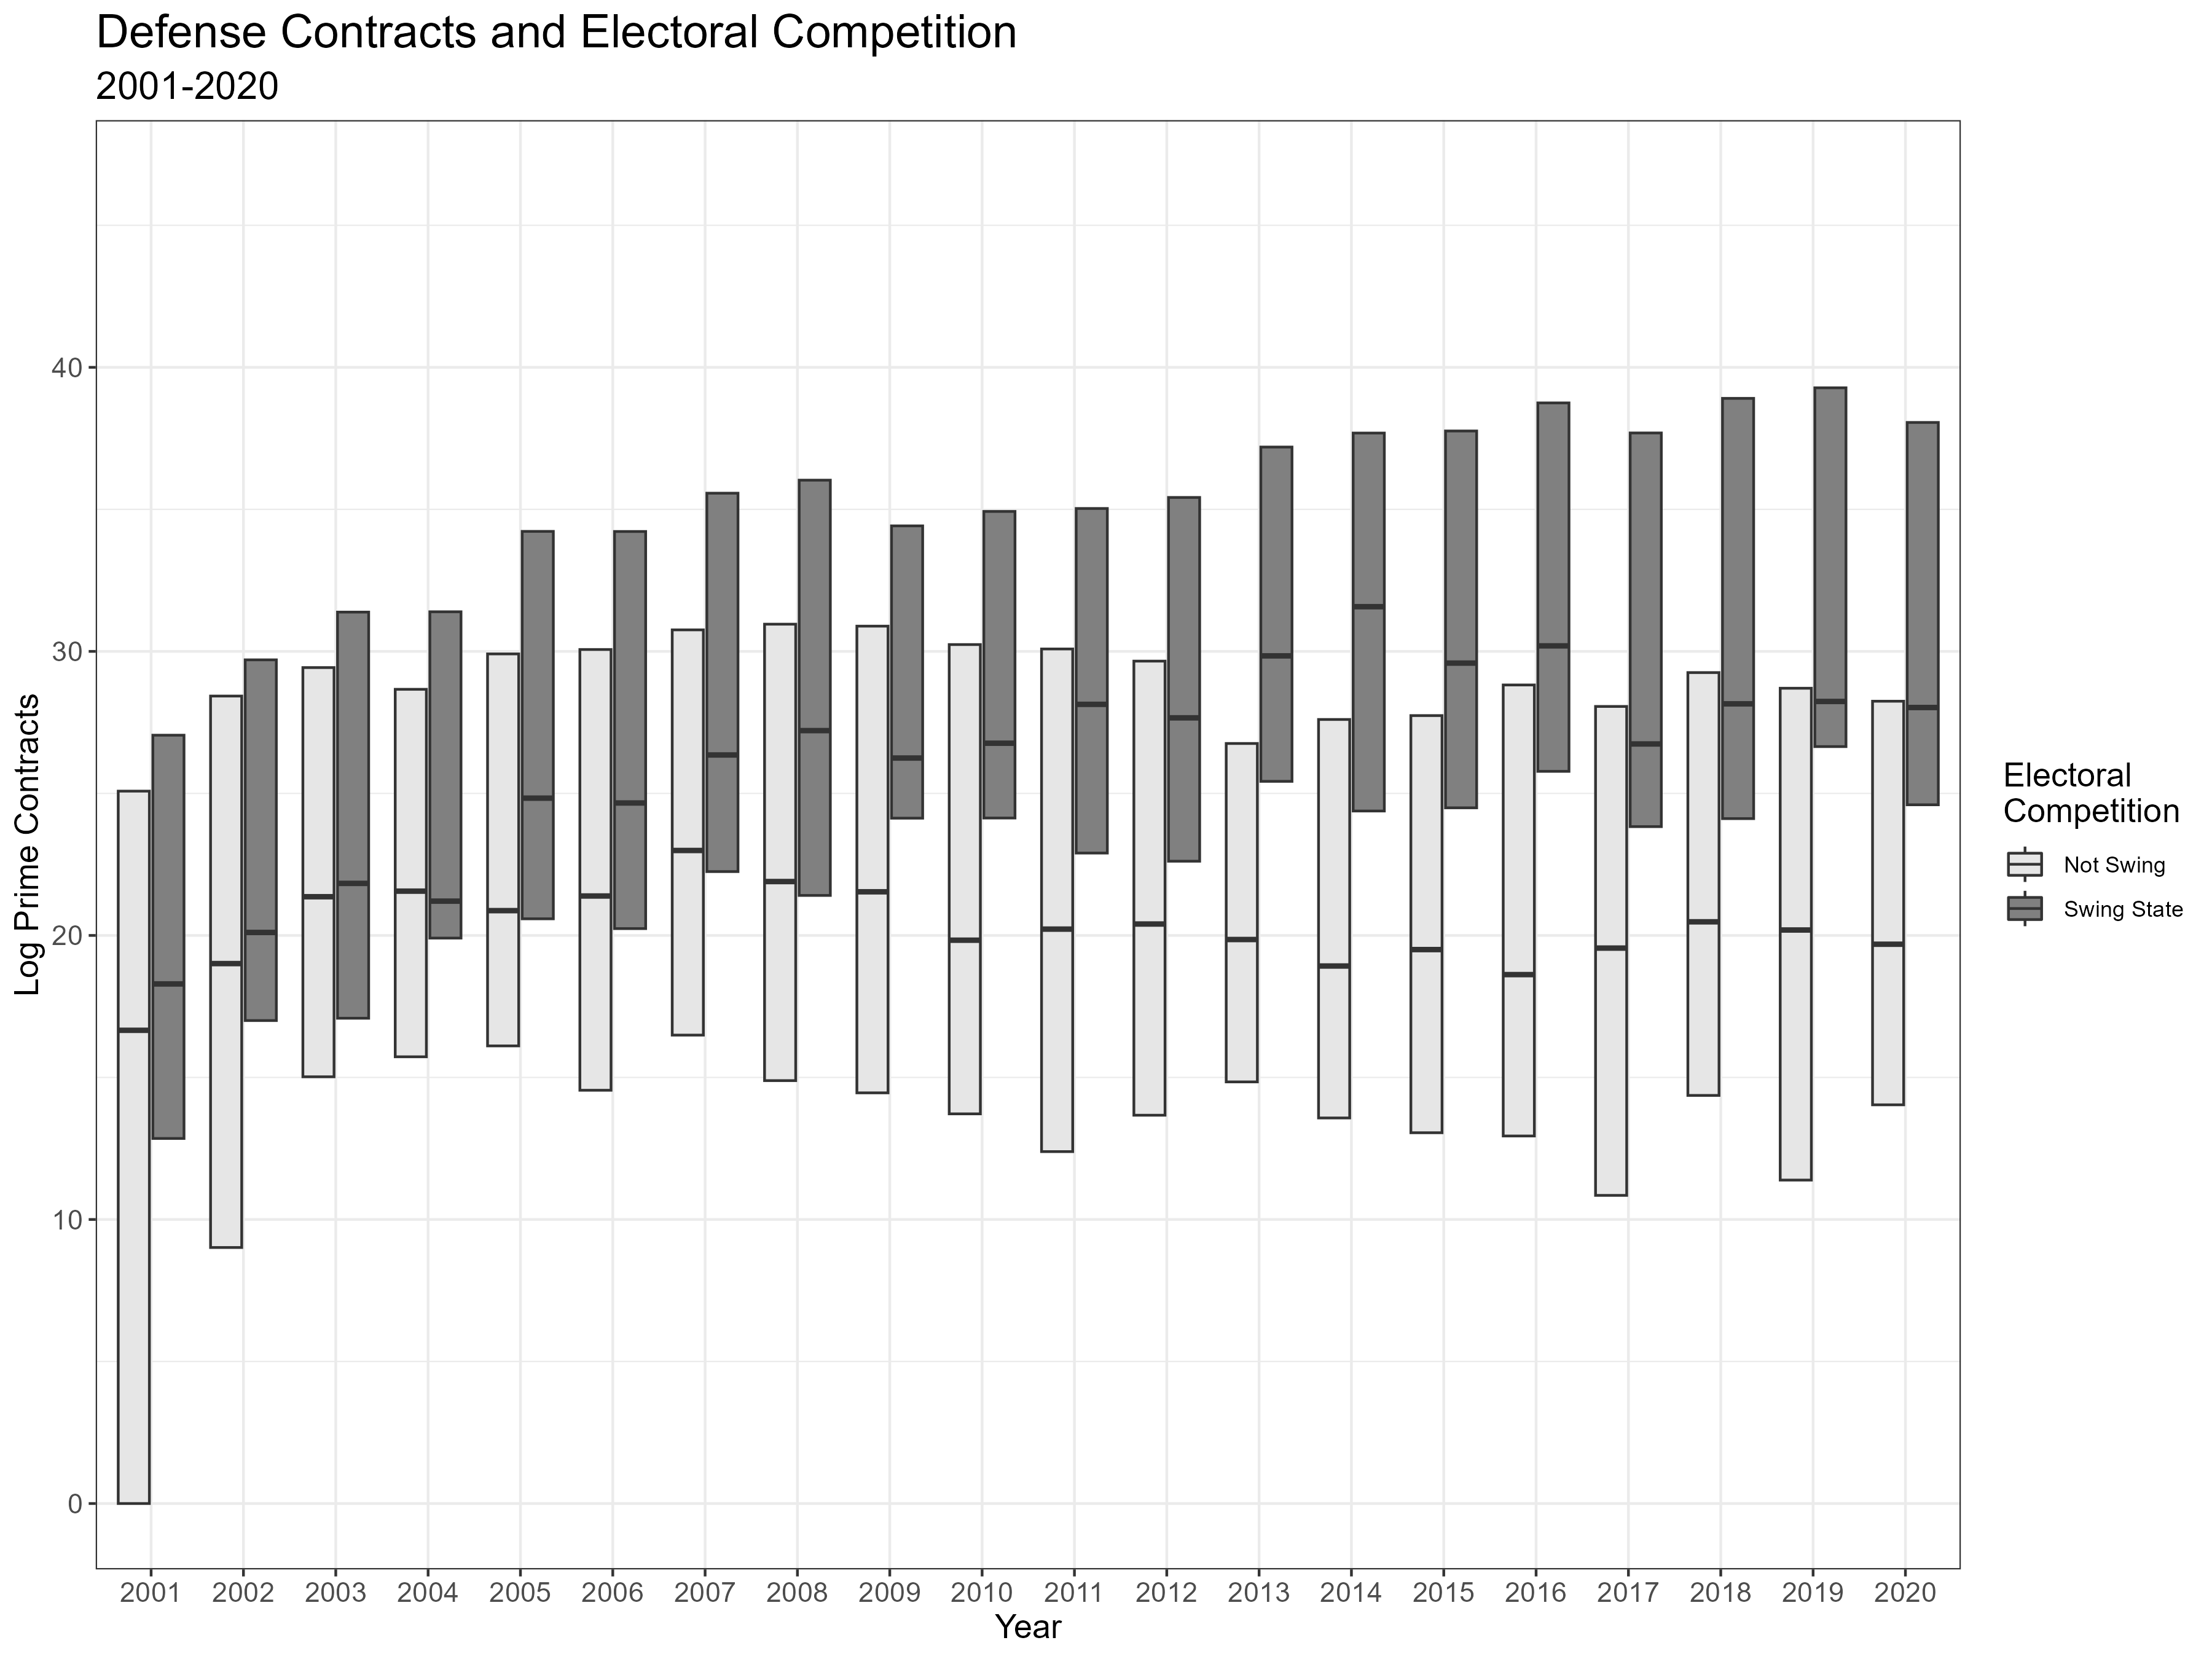
\includegraphics[width=0.95\textwidth]{../figures/raw-comp-state.png}
	\caption{Raw distribution of prime defense contracts in swing and non-swing states, 2001-2020. The box plots show the median for each group and the interquartile range, which runs from the first to third quartile.}
	\label{fig:raw-comp-state}
\end{figure}


The distributional model tests an alternative expression of this argument and checks whether the patterns in the raw data hold after adjusting for state-level differences, temporal autocorrelation, and clustered observations.
As \autoref{fig:coef-comp-state} shows, the distributional model results support the contracts hypothesis as well.\footnote{Plots of state-specific autocorrelation as well as the state and year varying intercepts are available in the appendix.}
Compared to non-swing states in peacetime, swing states receive more defense contracts.
The expected difference of .8 on the log scale is roughly \$2.2 billion in defense contracts, not counting any long-run multipliers. 


\begin{figure}[htpb]
	\centering
		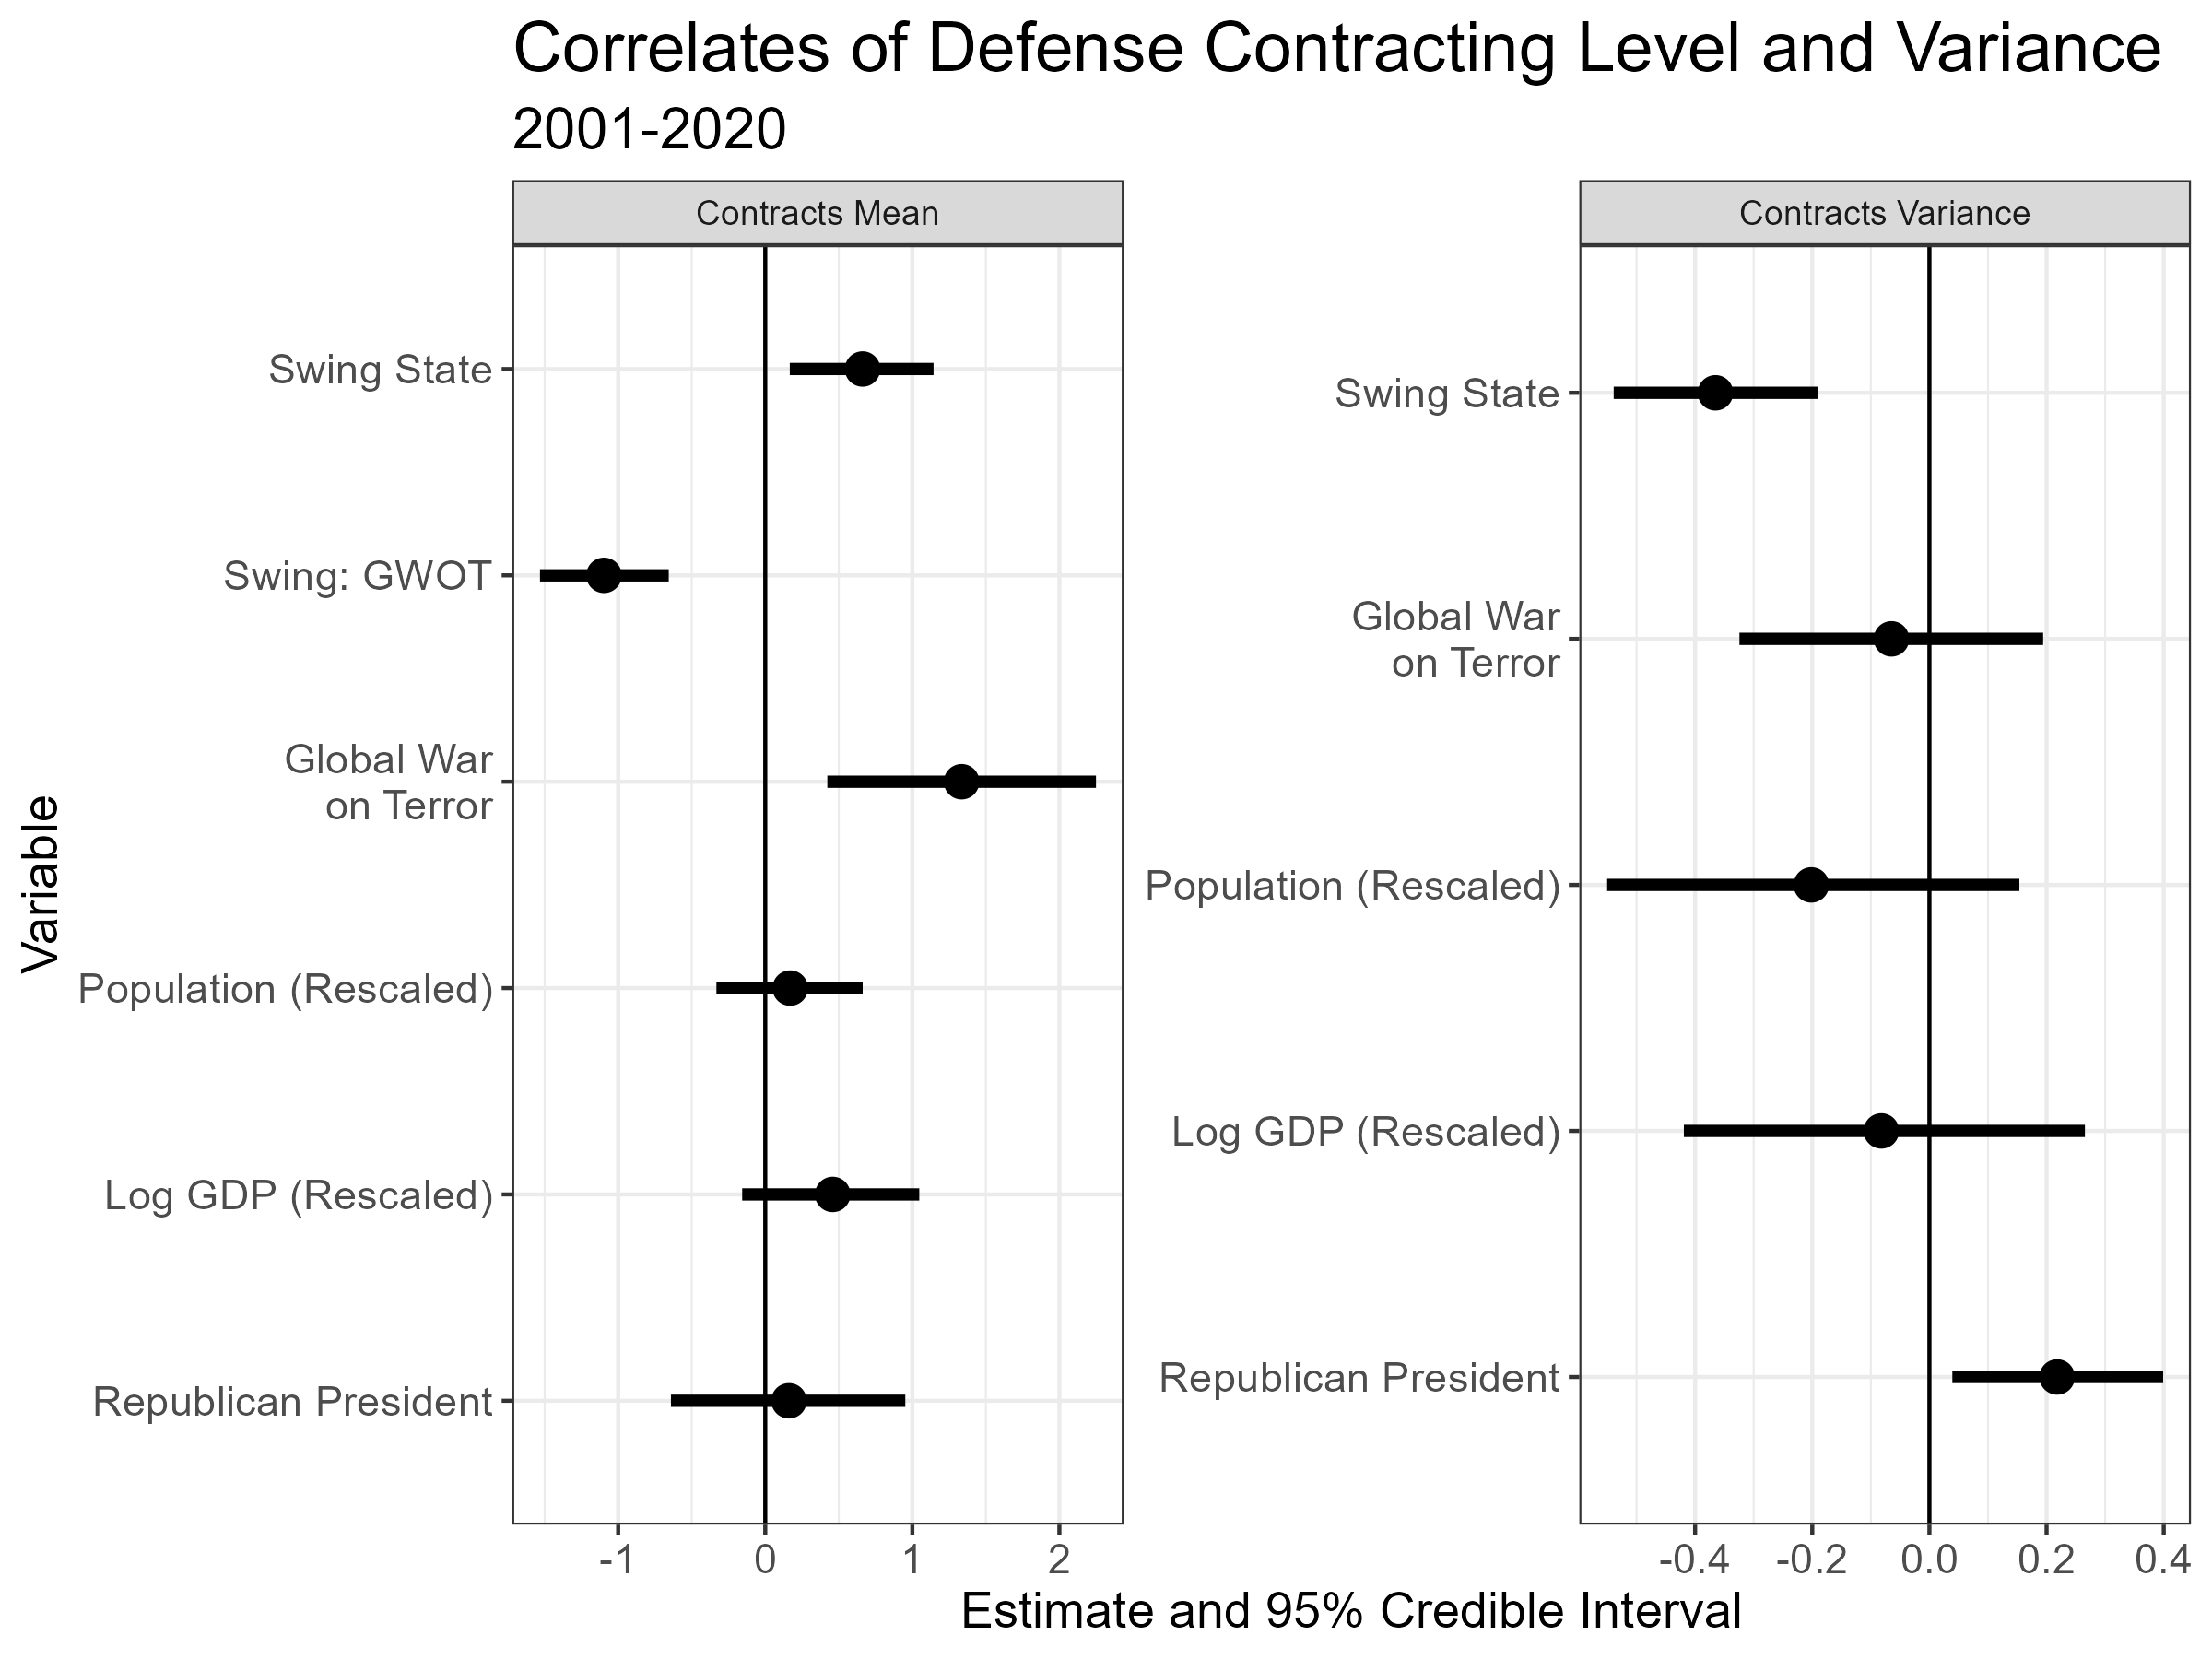
\includegraphics[width=0.95\textwidth]{../figures/coef-comp-state.png}
	\caption{Coefficient estimates from a distributional model of the mean and variance in prime contracting awards to U.S. states between 2001 and 2020. The first panel plots correlates of contract levels, and the second shows predictors of variation in contracts across states.}
	\label{fig:coef-comp-state}
\end{figure}


During the global war on terror, swing states received fewer contracts than other states, all else equal. 
This was partially because non-swing states received far more contracts during the most intense years of conflict, as the global war on terror coefficient indicates. 
In expectation, non-swing states received 1.32 more contract dollars on the log scale, which translates to roughly \$3.75 billion. 


Swing states also have less variation in contract awards than other states. 
The relationship shows up most clearly outside of the global war on terror. 
At the same time, the association between swing status and contract variance is of similar magnitude during the global war on terror, but this estimate has much more uncertainty. 
While it increased contract award levels the global war on terror did not change contract variance among non-swing states. 


None of the three controls are clearly correlated with contract levels. 
While the log GDP estimate is largely positive, it includes some small negative values as well. 
Republican presidents do not impact the mean of contract awards, but their presidencies are associated with greater variance in contracting. 


These estimates support the defense contracts hypothesis. 
In peacetime, swing states receive more defense contracts, and contract awards to these states are more consistent.  
In the final analysis, I examine how arms deals contribute to this relationship.




\section{A Bayesian Model of Contracts, Arms Exports, and Trade}


The two individual analyses provide initial support for the argument, but they also treat each part of the process in isolation. 
To show the full process, I employ a generative model where each stage of the process informs the next level.
This move 
I employ this approach because standard multiple-equation models in political science cannot easily accommodate divergent levels of analysis.
Flexible structure and Bayesian estimation can capture a wide variety of complex data-generating structures, subject to careful model validation \citep{Betancourt2021}. 





\section{Discussion and Conclusion}


The argument and results suggest that political budget and defense contracting cycles expand international trade, especially arms exports to U.S. allies. 
Economic efforts to bolster presidential electoral prospects have international consequences. 
Additional goods from defense contracting cycles produce arms flows outside the United States.
This bolsters cooperative relations between the United States and its allies.


Allied economic and security statecraft thus helps U.S. leaders win elections. 
While this is not a part of formal alliance bargains, these informal linkages are essential to grand bargains between alliance patrons and prot{\'e}g{\'e}s.
Allies need not undertake these cycles deliberately, but their accepting arms transfers is part of a cooperative bundle of ties regardless.


Allied support for political budget cycles affects democratic alliance credibility and maintenance. 
A stable alliance bargain can develop if leaders anticipate the electoral benefits of defense contracting cycles and arms exports to allies.
When leaders expect that maintaining security commitment will have electoral rewards, they will be more likely to invest in alliances. 


These findings also add an international security component to the political budget cycle literature.
Alliance partnerships can allow leaders to manipulate economic conditions for electoral gain. 
By providing an outlet for defense contracting , allies help leaders contract for new goods with less attention to the absorptive capacity and force planning of the U.S. military.


Finally, the argument and findings add to prior findings that states manipulate international economic and security cooperation to bolster or undermine leaders. 
To give one example, \citet{ChyzhUrbatsch2021} show that Chinese soy tariffs reduced support for Republicans in the 2018 midterm elections. 
Allies have both motive and means to use economic and security cooperation to help leaders. 
Rather than undermine leaders, allied arms import decisions create positive inducements for regular cooperation.


Future research could proceed in several directions. 
First, cycles in other economic outcomes such as foreign direct investment, are an interesting area for study. 
Exploring the role of defense industry integration and intermediate goods in these arms cycles is also critical.
Whether these results generalize to autocratic alliances or other democratic alliance patrons is another worthwhile inquiry. 
Security partners of other alliance patrons may take similar actions in different industries, for instance.


In conclusion, political budget cycles reshape international economic and security cooperation.
Budget cycles increase trade and arms transfers to U.S. allies through economic growth and defense contracting.
Security cooperation can therefore facilitate electoral benefits for leaders. 


\newpage
\singlespace
 
\bibliography{../../MasterBibliography} 


\end{document}
